\documentclass{beamer}
\usepackage{ctex, hyperref}
\usepackage[T1]{fontenc}

% other packages
\usepackage{latexsym,amsmath,xcolor,multicol,booktabs,calligra}
\usepackage{graphicx,pstricks,listings,stackengine}
\usepackage[normalem]{ulem}

\author{userElaina}
\title{When LLMs Meet Vector Databases}
\institute{School of AI}
\date{2024.06.01}
\usepackage{JilinUniv}

\def\cmd#1{\texttt{\color{red}\footnotesize $\backslash$#1}}
\def\env#1{\texttt{\color{blue}\footnotesize #1}}
\definecolor{deepblue}{rgb}{0,0,0.5}
\definecolor{deepred}{rgb}{0.6,0,0}
\definecolor{deepgreen}{rgb}{0,0.5,0}
\definecolor{halfgray}{gray}{0.55}

\lstset{
    basicstyle=\ttfamily\small,
    keywordstyle=\bfseries\color{deepblue},
    emphstyle=\ttfamily\color{deepred},    % Custom highlighting style
    stringstyle=\color{deepgreen},
    numbers=left,
    numberstyle=\small\color{halfgray},
    rulesepcolor=\color{red!20!green!20!blue!20},
    frame=shadowbox,
}

\begin{document}

\kaishu
\begin{frame}
    \titlepage
    \begin{figure}[htpb]
        \begin{center}
            
\includegraphics[width=0.15\linewidth]{pic/Jilin_University_Logo.eps}
        \end{center}
    \end{figure}
\end{frame}

\begin{frame}
\tableofcontents[sectionstyle=show,subsectionstyle=show/shaded/hide,subsubsectionstyle=show/shaded/hide]
\end{frame}

\section{Large Language Models}

\begin{frame}{challenges}
    \begin{itemize}
        \item Hallucinations (幻觉问题)
        \item Oblivion (记忆问题)
        \item Multimodal
        \item Security and ...
    \end{itemize}
\end{frame}

\section{Vector Databases}

\begin{frame}{Vector Databases, 向量数据库}
    \begin{itemize}
        \item 设计用于处理高维向量数据
        \item 把数据转化成向量(而不是表格)的形式, 存储在向量空间内
        \item 近似最近邻 (Approximate Nearest Neighbor, ANN)
        \item Multimodal
        \item 索引, 搜索加速, 可扩展性, 存储优化, 实时性, 灵活性, ...
    \end{itemize}
\end{frame}

\section{Retrieval Augmented Generation}

\begin{frame}{架构}
    \begin{figure}[c]
        \centering
        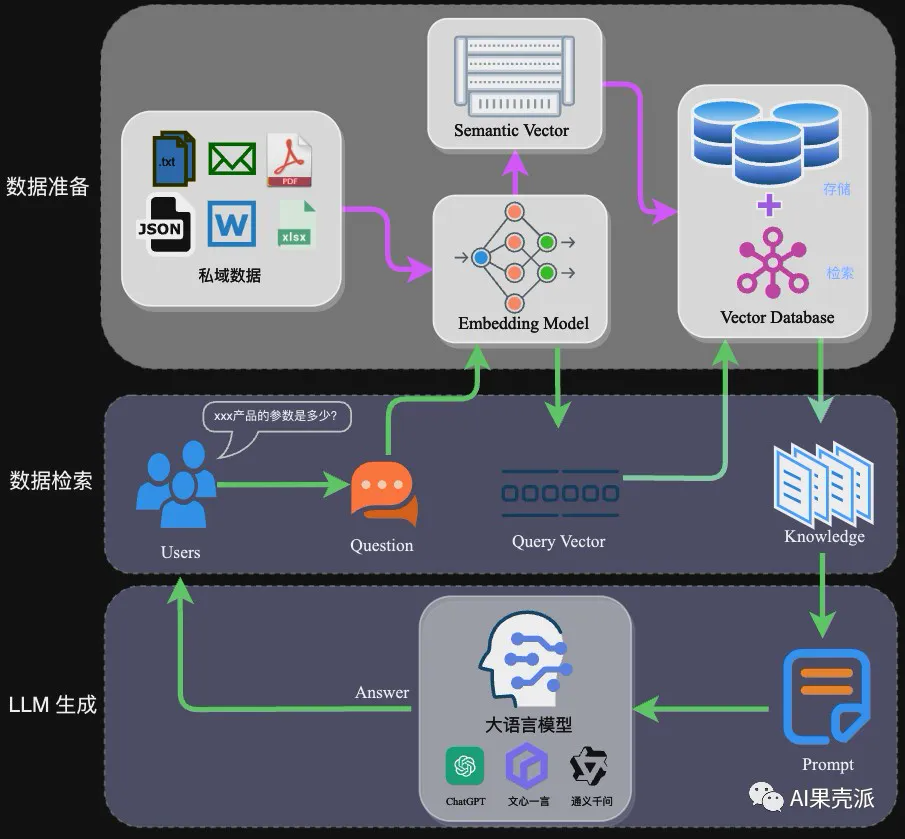
\includegraphics[height=.75\textheight]{pic/1.png}
        \caption{RAG, Retrieval Augmented Generation, 检索增强生成}
    \end{figure}
\end{frame}

\begin{frame}{Prompt}
    \tt
    【任务描述】\\
    假如你是一个专业的客服机器人,请参考【背景知识】,回回答问题 \\
    【背景知识】\\
    \{\{数据检索得到的相关文本\}\} \\
    【问题】\\
    xx-xx型号产品的xxx参数是多少?\\
\end{frame}

\begin{frame}{发展}
    \begin{itemize}
        \item 多租户
        \item 成本: 蒸馏, ...
        \item 向量化: Multimodal, 预处理, ...
        \item 向量数据库: ANN, 传统数据库, ...
    \end{itemize}
\end{frame}

\begin{frame}{Q \& A}
    \begin{center}
        {\Huge\calligra Thanks!}
    \end{center}
\end{frame}

\end{document}
